Subbab ini mendokumentasikan rancangan eksperimen yang dilaksanakan dalam penelitian ini, mencakup deskripsi delapan skenario pengujian, prosedur pelaksanaan setiap \textit{trial}, parameter eksperimen yang digunakan, dan panduan replikasi. Dokumentasi ini disusun untuk memastikan bahwa hasil penelitian dapat direproduksi secara independen~\cite{Adiuku2024}.

% -----------------------------------------------------------------------
\subsection{Lingkungan dan Skenario Pengujian}
\label{sec:skenario}
% -----------------------------------------------------------------------

Seluruh pengujian dilaksanakan dalam lingkungan simulasi berbasis Gazebo dengan peta lingkungan \textit{indoor} bertopologi koridor dan ruangan (\texttt{grit\_1\_edited\_2.yaml}, resolusi 0,05~m/sel). Setiap skenario menggunakan \textit{world file} Gazebo yang berbeda, namun peta navigasi dan konfigurasi sensor tetap identik pada seluruh skenario. Titik awal robot ditetapkan pada koordinat $(0, 0)$ dan titik tujuan pada $(9{,}159;\ 6{,}240)$ untuk delapan skenario yang diuji.

Delapan skenario disusun dalam empat pasang (\textit{paired design}), di mana setiap pasangan menguji kondisi lingkungan yang sama tetapi dengan dua konfigurasi berbeda, yaitu \textit{baseline} tanpa fuzzy (S1--S4) dan \textit{proposed method} dengan fuzzy (S5--S8). Desain berpasangan ini memungkinkan perbandingan langsung antara kedua konfigurasi menggunakan uji statistik non-parametrik Mann--Whitney U pada kondisi lingkungan yang identik (Subbab~\ref{sec:metode_statistik}).

\begin{table}[H]
\centering
\caption{Deskripsi delapan skenario pengujian. Setiap pasangan (S$n$/S$(n+4)$) menguji kondisi lingkungan yang sama dengan konfigurasi kontrol berbeda.}
\label{tab:skenario_pengujian}
\begin{tabular}{cllll}
\toprule
\textbf{Sk.} & \textbf{World File} & \textbf{Obstacle} &
\textbf{Fuzzy} & \textbf{Aspek yang Diuji} \\
\midrule
S1 & \texttt{S1\_open.world}           & Tidak ada         & Tidak & Baseline navigasi murni \\
S2 & \texttt{S2\_single\_human.world}  & 1 statis (human)  & Tidak & Baseline satu obstacle \\
S3 & \texttt{S3\_static\_multi.world}  & Multi statis + kucing & Tidak & Baseline \textit{blind-spot} \\
S4 & \texttt{S4\_dynamic\_multi.world} & Multi dinamis + kucing & Tidak & Baseline dinamis \\
\midrule
S5 & \texttt{S1\_open.world}           & Tidak ada         & Ya & Efek fuzzy tanpa obstacle \\
S6 & \texttt{S2\_single\_human.world}  & 1 statis (human)  & Ya & Efek fuzzy satu obstacle \\
S7 & \texttt{S3\_static\_multi.world}  & Multi statis + kucing & Ya & Fuzzy pada \textit{blind-spot} \\
S8 & \texttt{S4\_dynamic\_multi.world} & Multi dinamis + kucing & Ya & Fuzzy pada dinamis \\
\bottomrule
\end{tabular}
\end{table}

\subsubsection*{a. Skenario S1/S5 --- Navigasi Tanpa Obstacle}

Skenario S1 dan S5 menggunakan lingkungan \texttt{S1\_open.world} yang tidak mengandung obstacle aktif selain dinding dan struktur peta statis. Skenario ini berfungsi sebagai \textit{control condition} untuk mengisolasi efek logika fuzzy terhadap pola navigasi robot pada kondisi bebas gangguan. Pada S5, \textit{fuzzy controller} aktif meskipun tidak ada obstacle terdekat, sehingga $d_\text{obs}$ selalu tinggi dan $\tau_\text{eff} \approx 1{,}0$; sesuai basis aturan, robot diizinkan bergerak dengan kecepatan penuh dan gain lemah. Selisih kecepatan dan panjang lintasan antara S1 dan S5 menjadi indikator \textit{overhead} yang ditimbulkan fuzzy pada kondisi normal.

\subsubsection*{b. Skenario S2/S6 --- Satu Obstacle Statis}

Skenario S2 dan S6 menggunakan lingkungan \texttt{S2\_single\_human.world} yang memuat satu \textit{obstacle} manusia statis (silinder $r = 0{,}25$~m, tinggi 3~m, posisi $(2{,}466;\ 1{,}273)$~m) yang dapat dideteksi oleh LiDAR. Skenario ini menguji kemampuan dasar penghindaran \textit{obstacle} konvensional serta efek logika fuzzy terhadap \textit{clearance} pada kondisi \textit{obstacle} tunggal. Tidak terdapat \textit{obstacle} kucing pada skenario ini.

\subsubsection*{c. Skenario S3/S7 --- Obstacle Majemuk Statis dengan Kucing}

Skenario S3 dan S7 merupakan skenario utama yang menguji hipotesis penelitian, yaitu apakah sistem mampu menghindari \textit{obstacle} kucing yang tidak terdeteksi LiDAR. Lingkungan \texttt{S3\_static\_multi.world} memuat tiga \textit{obstacle} statis, yaitu: (a) satu \textit{obstacle} statis standar ($r = 0{,}25$~m), (b) \texttt{obstacle\_cat} ($r = 0{,}18$~m, tinggi $\approx$0,19~m, posisi $(2{,}83;\ 0{,}97)$~m) yang berada di \textit{blind-spot} LiDAR, dan (c) dua \textit{obstacle\_human} statis ($r = 0{,}25$~m, tinggi 3~m). Pasangan S3/S7 memungkinkan perbandingan \textit{clearance} terhadap kucing antara konfigurasi \textit{baseline} dan fuzzy dalam kondisi yang terkontrol.

\subsubsection*{d. Skenario S4/S8 --- Obstacle Majemuk Dinamis dengan Kucing}

Skenario S4 dan S8 menambahkan lapisan kompleksitas dengan menggerakkan kedua \textit{obstacle} manusia secara osilasi mulus menggunakan skrip \texttt{dynamic\_obstacles.py}. Masing-masing \textit{obstacle} manusia bergerak bolak-balik di sepanjang jalur linear: human\_1 menempuh jalur sepanjang $\approx 3{,}07$~m dan human\_2 sepanjang $\approx 3{,}23$~m, keduanya dengan profil kecepatan sinusoidal yang menghasilkan kecepatan puncak masing-masing $\approx 0{,}77$~m/s dan $\approx 0{,}81$~m/s. Gerak osilasi dimodelkan menggunakan fungsi:
\begin{equation}
    s(t) = \frac{1}{2}\bigl(1 - \cos(\omega t)\bigr),
    \quad \omega = 0{,}5~\text{rad/s}
    \label{eq:osilasi_human}
\end{equation}
di mana $s(t) \in [0, 1]$ adalah parameter posisi ternormalisasi di sepanjang jalur masing-masing \textit{obstacle} ($s=0$: titik A, $s=1$: titik B). Fungsi kosinus terbalik ini menghasilkan gerakan yang halus dengan akselerasi dan deselerasi di kedua ujung jalur, sehingga menghindari perubahan kecepatan mendadak yang tidak realistis. Posisi \textit{obstacle} diperbarui melalui layanan \texttt{/gazebo/set\_model\_state} pada frekuensi 50~Hz.

Fase gerak \textit{obstacle} tidak direset antar-\textit{trial}, sehingga setiap \textit{trial} mengalami kondisi pertemuan yang berbeda dan lebih mendekati variasi alami yang diharapkan pada penerapan nyata. Posisi kucing (\texttt{obstacle\_cat}) pada S4 terdapat sedikit \textit{offset} dibandingkan S3 ($\Delta x \approx 0{,}14$~m, $\Delta y \approx 0{,}003$~m) karena perbedaan \textit{world file}, tetapi perbedaan ini tidak mengubah karakteristik \textit{blind-spot}-nya secara substansial.

Pada skenario S4 dan S8, mekanisme \textit{dynamic prediction} dan \textit{temporal yield} juga aktif (Subbab~\ref{sec:obstacle_dinamis}), sebagai respons terhadap karakteristik \textit{obstacle} yang bergerak dengan kecepatan mendekati 0,8~m/s. Parameter APF yang berbeda dari skenario lain ($d_0 = 1{,}20$~m, \texttt{obs\_detect\_radius} = 1,30~m) juga hanya berlaku pada S4 dan S8 untuk memberikan jarak reaksi yang lebih awal terhadap \textit{obstacle} dinamis.

\begin{figure}[H]
    \centering
    \begin{minipage}{0.48\textwidth}
        \centering
        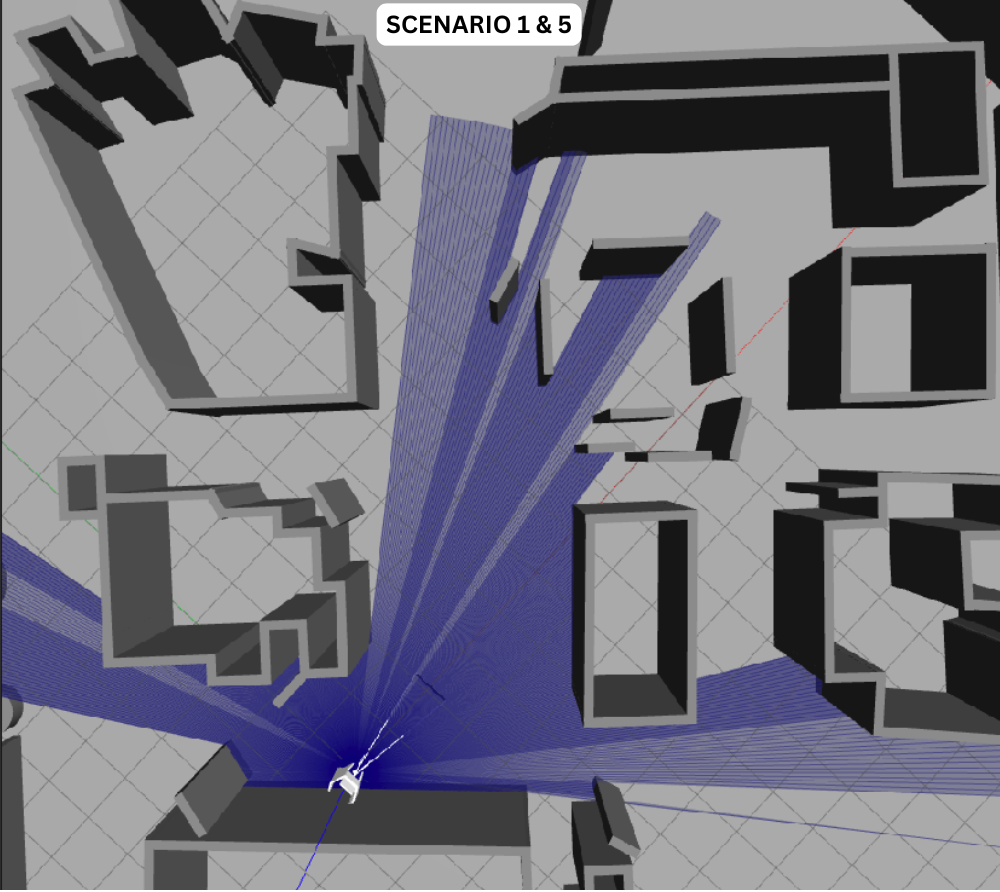
\includegraphics[width=\textwidth]{gambar/3.8_skenario_S1_S5.png}
        \\(a) S1/S5
    \end{minipage}
    \hfill
    \begin{minipage}{0.48\textwidth}
        \centering
        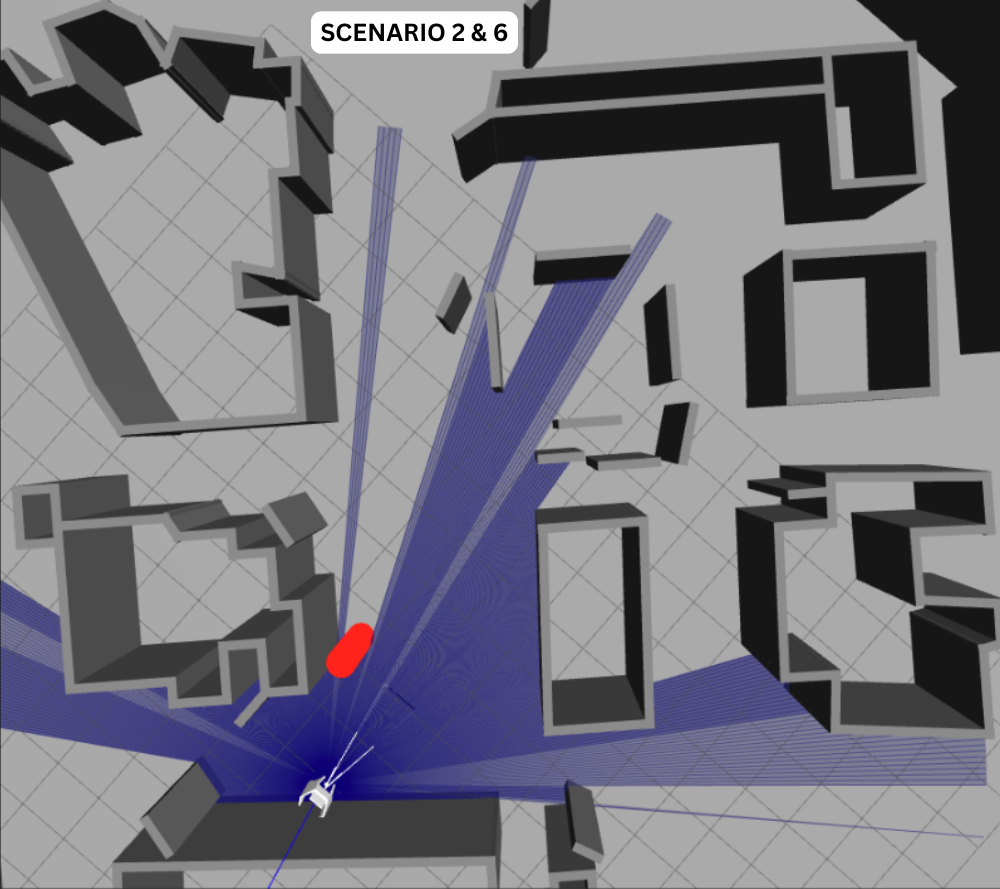
\includegraphics[width=\textwidth]{gambar/3.8_skenario_S2_S6.png}
        \\(b) S2/S6
    \end{minipage}

    \vspace{0.5em}

    \begin{minipage}{0.48\textwidth}
        \centering
        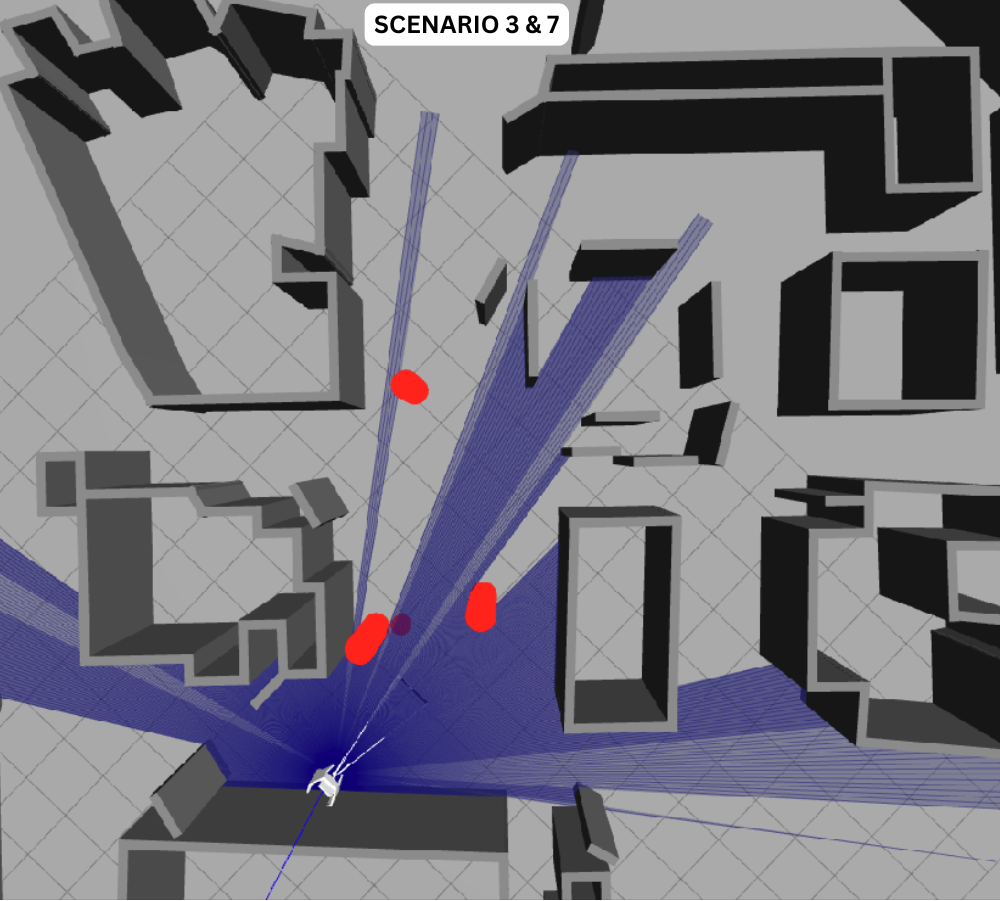
\includegraphics[width=\textwidth]{gambar/3.8_skenario_S3_S7.png}
        \\(c) S3/S7
    \end{minipage}
    \hfill
    \begin{minipage}{0.48\textwidth}
        \centering
        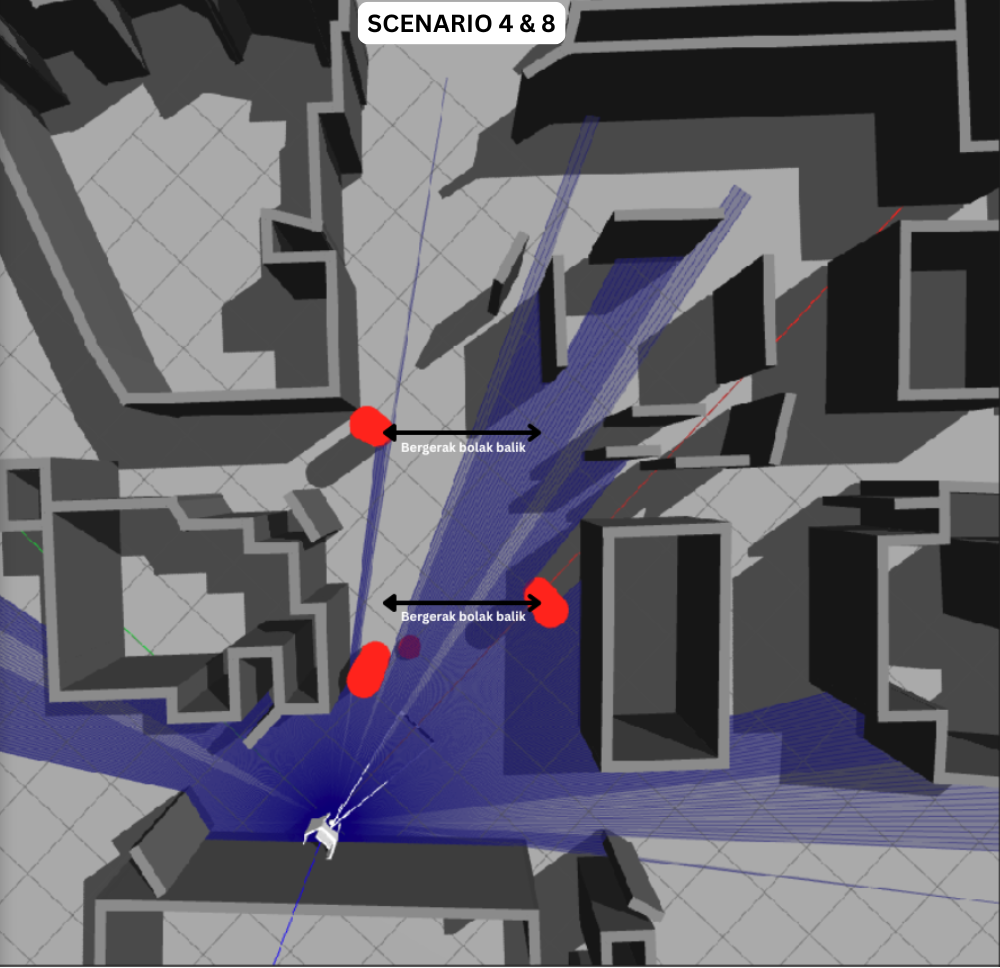
\includegraphics[width=\textwidth]{gambar/3.8_skenario_S4_S8.png}
        \\(d) S4/S8
    \end{minipage}
    \caption{Tampak atas empat lingkungan pengujian di Gazebo. Jalur biru menunjukkan jangkauan pindaian LiDAR \textit{real-time}; blob merah menandai sumber panas yang terdeteksi kamera termal. (a) S1/S5: tanpa \textit{obstacle} aktif. (b) S2/S6: satu \textit{obstacle} statis bersuhu tubuh. (c) S3/S7: tiga sumber panas (\textit{obstacle\_cat} dan dua \textit{obstacle\_human}) dari total empat \textit{obstacle} fisik; satu \textit{obstacle} statis tambahan tidak terdeteksi termal karena tidak bersuhu tubuh. (d) S4/S8: dua \textit{obstacle\_human} bergerak osilasi (ditandai panah \textit{"Bergerak bolak balik"}), sedangkan \textit{obstacle\_cat} tetap statis.}
    \label{fig:skenario_panel}
\end{figure}

\begin{figure}[H]
    \centering
    \begin{minipage}{0.48\textwidth}
        \centering
        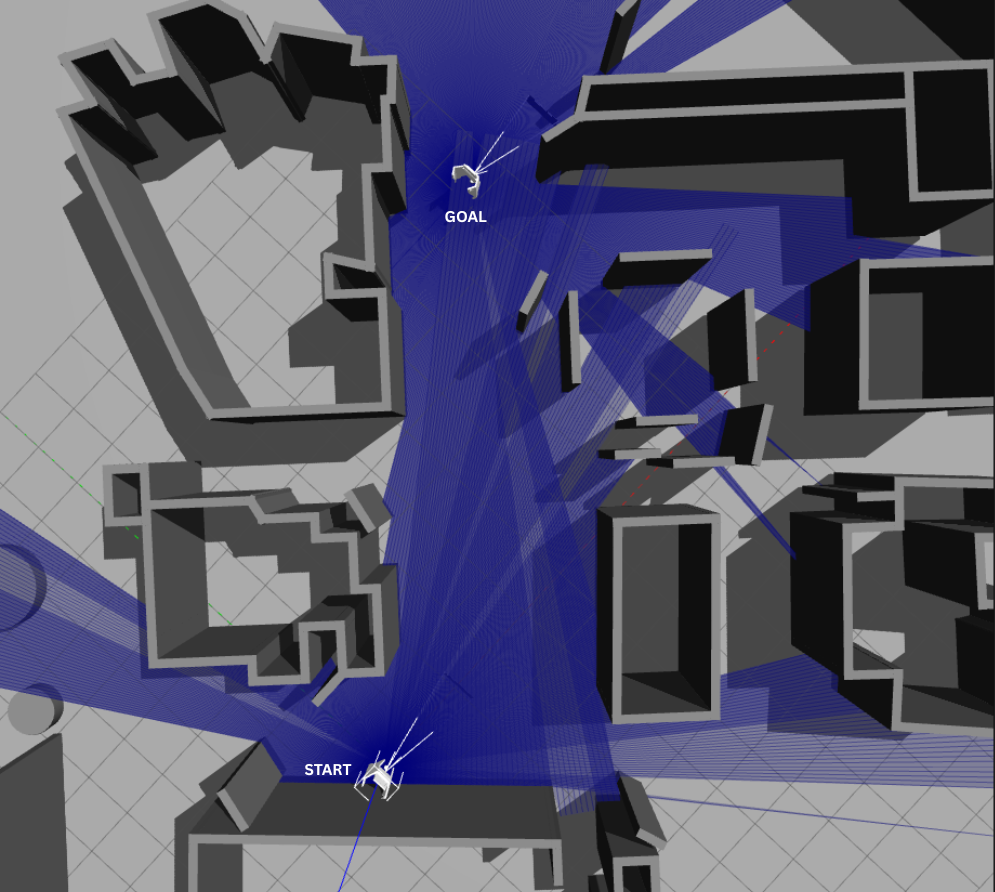
\includegraphics[width=\textwidth]{gambar/3.8_map_gazebo.png}
        \\(a) Tampak atas Gazebo
    \end{minipage}
    \hfill
    \begin{minipage}{0.48\textwidth}
        \centering
        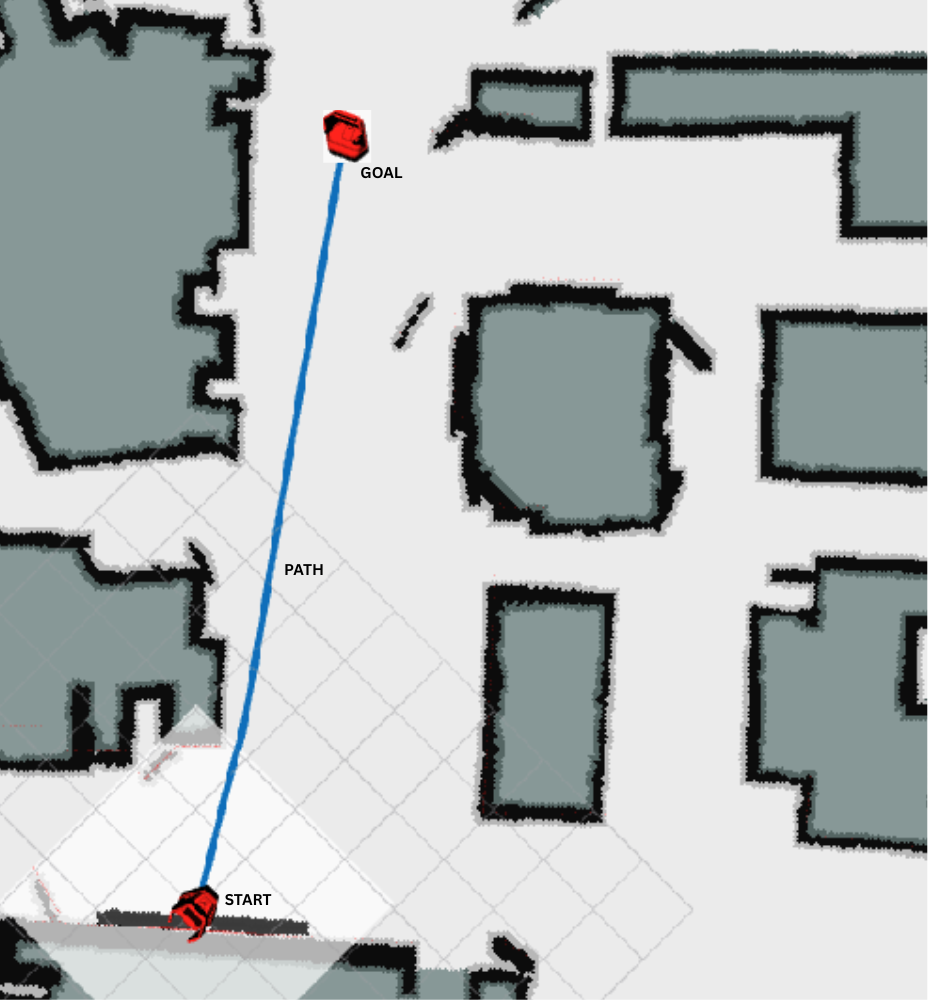
\includegraphics[width=\textwidth]{gambar/3.8_map_rviz.png}
        \\(b) Representasi RViz
    \end{minipage}
    \caption{Konfigurasi titik awal (START) dan tujuan (GOAL) yang identik untuk seluruh delapan skenario pengujian. (a) Tampak atas pada simulator Gazebo, menunjukkan kompleksitas geometris lingkungan \textit{indoor}. (b) Representasi pada RViz menggunakan peta \texttt{grit\_1\_edited\_2} (\textit{occupancy grid}), dengan garis biru menunjukkan jalur global yang dihasilkan NavfnROS sebelum eksekusi \textit{trial}. Koordinat \textit{frame} peta: START $= (0, 0)$, GOAL $= (9{,}159;\ 6{,}240)$.}
    \label{fig:map_annotated}
\end{figure}

% -----------------------------------------------------------------------
\subsection{Prosedur Eksperimen}
\label{sec:prosedur}
% -----------------------------------------------------------------------

Setiap skenario dijalankan sebanyak $n = 10$ \textit{trial} secara berurutan menggunakan skrip otomatis \texttt{run\_trials.py}. Pemilihan $n = 10$ didasarkan pada keterbatasan komputasi dan waktu simulasi, serta kecukupan untuk uji Mann--Whitney U pada kasus dengan \textit{effect size} besar yang diantisipasi dari desain sistem~\cite{PerezHigueras2023}.

\subsubsection*{a. Urutan Pelaksanaan}

Prosedur untuk setiap skenario mengikuti urutan berikut:

\begin{enumerate}
    \item \textbf{Persiapan lingkungan:} \textit{workspace} di-\textit{source} dan \textit{launch file} utama dijalankan dengan argumen skenario:
    \begin{center}
    \texttt{roslaunch ros\_sim nav\_sim.launch scenario:=S$x$}
    \end{center}
    \textit{Launch file} ini menginisialisasi Gazebo, semua \textit{node} ROS (termasuk pipeline termal, APFPlanner, \textit{move\_base}, dan \textit{fake\_localization}), serta menetapkan parameter APF dan fuzzy sesuai skenario.

    \item \textbf{Aktivasi obstacle dinamis (khusus S4/S8):} Setelah simulasi stabil, skrip \texttt{dynamic\_obstacles.py} dijalankan di terminal terpisah untuk memulai gerak osilasi kedua \textit{obstacle} manusia. Skrip ini terus berjalan sepanjang durasi 10 \textit{trial} tanpa direset antartial, sehingga fase gerak manusia berlanjut secara alami dan memberikan variasi kondisi pertemuan yang lebih realistis.

    \item \textbf{Pencatatan data:} \textit{Node} \texttt{experiment\_logger.py} dijalankan secara paralel untuk mencatat metrik setiap \textit{trial} ke berkas CSV.

    \item \textbf{Pelaksanaan batch trial:} Skrip \texttt{run\_trials.py} dijalankan dengan parameter skenario dan jumlah \textit{trial}:
    \begin{center}
    \texttt{rosrun fuzzy\_thermal\_nav run\_trials.py \_scenario:=S$x$ \_n:=10}
    \end{center}
    Skrip ini secara otomatis mengeksekusi siklus setiap \textit{trial}.
\end{enumerate}

\subsubsection*{b. Prosedur Setiap \textit{Trial}}

Untuk setiap \textit{trial} ke-$i$ dari $n = 10$, \texttt{run\_trials.py} melakukan langkah berikut secara berurutan:

\begin{enumerate}
    \item \textbf{Reset posisi robot:} Robot dikembalikan ke posisi awal $(0, 0)$ menggunakan layanan \texttt{/gazebo/set\_model\_state} dengan kecepatan nol (\textit{twist zeroed}). Karena robot menggunakan model kinematik \texttt{libgazebo\_ros\_planar\_move}, pose odometri mengikuti pose model sehingga \textit{fake\_localization} secara otomatis memperbarui posisi dalam \textit{frame} peta.

    \item \textbf{Delay stabilisasi:} Penundaan 1~detik diberikan setelah reset posisi untuk memastikan topik odometri stabil sebelum langkah berikutnya.

    \item \textbf{Pembersihan \textit{costmap}:} Layanan \texttt{/move\_base/clear\_costmaps} dipanggil untuk menghapus semua penanda \textit{obstacle} yang tersisa dari \textit{trial} sebelumnya, diikuti penundaan \texttt{settle = 2{,}0}~detik untuk memastikan \textit{costmap} terisi ulang dari data sensor terkini. Langkah ini memastikan setiap \textit{trial} dimulai dari representasi lingkungan yang baru.

    \item \textbf{Pengiriman \textit{goal}:} \textit{Goal} dikirimkan ke \texttt{/move\_base\_simple/goal} pada koordinat $(9{,}159;\ 6{,}240)$ dengan orientasi $q_z = 0{,}086$ dan $q_w = 0{,}997$.

    \item \textbf{Pemantauan dan \textit{timeout}:} Skrip memantau topik \texttt{/move\_base/result} untuk mendapatkan status penyelesaian. \textit{Trial} dinyatakan selesai ketika status diterima (sukses: kode 3; gagal/dibatalkan: kode 4), atau apabila durasi telah melampaui batas waktu maksimum \texttt{max\_time = 120}~detik (\textit{timeout}). \textit{Trial} yang berakhir karena \textit{timeout} dicatat sebagai gagal.

    \item \textbf{Pencatatan hasil:} \texttt{experiment\_logger.py} mendeteksi akhir \textit{trial} melalui topik yang sama, kemudian menuliskan ringkasan metrik ke berkas \texttt{results\_S$x$.csv}.
\end{enumerate}

Setelah 10 \textit{trial} selesai, hasil CSV dianalisis menggunakan skrip \texttt{analyze\_results.py} dan visualisasi lintasan dihasilkan menggunakan \texttt{plot\_trajectories.py} (untuk skenario statis) atau \texttt{Plot\_trajectories\_dynamic.py} (untuk S4/S8). Kedua skrip tersebut dijalankan secara \textit{offline} setelah eksperimen selesai.

% -----------------------------------------------------------------------
\subsection{Parameter Eksperimen}
\label{sec:param_eksperimen}
% -----------------------------------------------------------------------

Tabel~\ref{tab:param_eksperimen} merangkum seluruh parameter utama yang digunakan dalam eksperimen, dibagi berdasarkan kategori. Seluruh nilai ini diambil dari konfigurasi \textit{final} pada \texttt{nav\_sim.launch} dan tidak berubah selama pelaksanaan eksperimen kecuali yang ditandai khusus untuk S4/S8.

\begin{table}[H]
\centering
\caption{Parameter eksperimen final yang digunakan pada seluruh skenario. Nilai S4/S8 hanya berlaku untuk skenario dengan obstacle dinamis.}
\label{tab:param_eksperimen}
\begin{tabular}{llll}
\toprule
\textbf{Kategori} & \textbf{Parameter} & \textbf{Nilai} & \textbf{Keterangan} \\
\midrule
\multirow{4}{*}{Navigasi}
  & \texttt{controller\_frequency} & 10{,}0~Hz & Frekuensi kendali lokal \\
  & \texttt{planner\_frequency}    & 0{,}2~Hz  & Frekuensi \textit{replanning} global \\
  & Goal ($x$, $y$)                & (9{,}159; 6{,}240) & Koordinat tujuan (m) \\
  & \texttt{max\_time}             & 120~detik & Batas waktu per \textit{trial} \\
\midrule
\multirow{5}{*}{APF}
  & $k_\text{att}$     & 1,5     & Penguatan atraktif \\
  & $k_\text{rep}$     & 0,4     & Penguatan repulsif \\
  & $d_0$ (S1--S3, S5--S7)         & 0,85~m  & Jarak pengaruh tolak \\
  & $d_0$ (S4, S8)                  & 1,20~m  & Diperlebar untuk dinamis \\
  & $v_\text{max}$     & 0,2~m/s & Kecepatan linear maksimum \\
  & $r_\text{robot}$   & 0,20~m  & Radius \textit{inscribed} untuk \textit{clearance} \\
\midrule
\multirow{5}{*}{\textit{Cat Keep-out}}
  & $r_\text{cat}$               & 0,18~m & Radius kucing \\
  & $\delta_\text{margin}$       & 0,08~m & Margin aman tepi-ke-tepi \\
  & $D_\text{safe}$              & 0,535~m & Jarak aman pusat-ke-pusat \\
  & $\delta_\text{infl}$         & 0,18~m & Zona pengaruh \textit{keep-out} \\
  & $G_\text{cat}$               & 3,0    & Penguatan \textit{keep-out} \\
\midrule
\multirow{3}{*}{Proyeksi Termal}
  & $r_\text{near}$              & 0,25~m  & Jarak piksel bawah \\
  & $r_\text{far}$               & 0,85~m  & Jarak piksel atas ROI \\
  & \texttt{min\_blob\_px}       & 40~piksel & Luas blob minimal \\
\midrule
\multirow{3}{*}{Eksperimen}
  & Jumlah \textit{trial} ($n$)  & 10 per skenario & Total 80 \textit{trial} \\
  & \texttt{settle}              & 2,0~detik & Delay setelah \textit{clear costmap} \\
  & Reset delay                  & 1,0~detik & Delay setelah reset posisi \\
\bottomrule
\end{tabular}
\end{table}

% -----------------------------------------------------------------------
\subsection{Replikasi Eksperimen}
\label{sec:replikasi}
% -----------------------------------------------------------------------

Untuk meningkatkan reprodusibilitas, seluruh konfigurasi sistem dikunci dalam berkas \texttt{nav\_sim.launch}; tidak ada parameter yang diubah secara manual antarskenario selain argumen \texttt{scenario:=S$x$}. Artinya, menjalankan kembali perintah \texttt{roslaunch ros\_sim nav\_sim.launch scenario:=S3} secara deterministik menghasilkan konfigurasi yang persis sama dengan yang digunakan saat pengambilan data~\cite{Adiuku2024}.

\subsubsection*{a. Kebutuhan Perangkat Lunak}

Replikasi memerlukan:
\begin{itemize}
    \item Ubuntu 20.04 LTS,
    \item ROS Noetic (termasuk paket \texttt{move\_base}, \texttt{costmap\_2d}, \texttt{navfn}, \texttt{fake\_localization}, dan \texttt{map\_server}),
    \item Gazebo 11 (termasuk \texttt{hector\_gazebo\_thermal\_camera}),
    \item Python 3 dengan dependensi: \texttt{rospy}, \texttt{opencv-python}, \texttt{cv\_bridge}, \texttt{numpy}, \texttt{pandas}, \texttt{scipy}, dan \texttt{matplotlib}.
\end{itemize}

\subsubsection*{b. Struktur Workspace}

Workspace ROS (\texttt{final\_ws}) terdiri dari tiga paket utama:
\begin{itemize}
    \item \texttt{ros\_sim}: berisi APFPlanner (C++), \texttt{fuzzy\_controller.h}, \textit{launch file} utama, dan model URDF robot.
    \item \texttt{asr\_navigation}: berisi konfigurasi \textit{costmap}, \textit{world file} (S1--S4), peta (\texttt{grit\_1\_edited\_2}), dan parameter APF.
    \item \texttt{fuzzy\_thermal\_nav}: berisi seluruh \textit{node} Python (pipeline termal, runner, logger, analisis), \textit{world file} S1/S3 untuk referensi, dan skrip analisis data.
\end{itemize}

\subsubsection*{c. Langkah Menjalankan Eksperimen}

Satu siklus eksperimen penuh untuk skenario S$x$ dapat direplikasi dengan langkah berikut:

\begin{enumerate}
    \item \textbf{Sumber workspace:}
    \begin{center}
    \texttt{source \textasciitilde/TA/final\_ws/devel/setup.bash}
    \end{center}

    \item \textbf{Jalankan simulasi:}
    \begin{center}
    \texttt{roslaunch ros\_sim nav\_sim.launch scenario:=S$x$}
    \end{center}
    Tunggu hingga Gazebo dan seluruh \textit{node} siap.

    \item \textbf{(Hanya S4/S8) Aktifkan obstacle dinamis:} Di terminal terpisah:
    \begin{center}
    \texttt{rosrun fuzzy\_thermal\_nav dynamic\_obstacles.py}
    \end{center}

    \item \textbf{Jalankan batch trial:} Di terminal ketiga:
    \begin{center}
    \texttt{rosrun fuzzy\_thermal\_nav run\_trials.py \_scenario:=S$x$ \_n:=10}
    \end{center}

    \item \textbf{Analisis data:} Setelah 10 \textit{trial} selesai:
    \begin{center}
    \texttt{python3 analyze\_results.py ---data \textasciitilde/TA/final\_ws/experiment\_data}
    \end{center}
\end{enumerate}